\chapter{Einleitung}

% -------- Absatz (A1) mit Fußnote + Zitaten ----------
\begin{A1}
Lorem ipsum dolor sit amet, consectetur adipiscing elit. Sed non risus. 
Suspendisse\footnote{Dies ist eine Beispiel-Fußnote, die einen kurzen Hinweis liefert.} 
lectus tortor, dignissim sit amet, adipiscing nec, ultricies sed, dolor. 
Wie bereits in der Literatur betont wurde (vgl. \cite{knuth1984}; \cite{meyer2012}), 
ist eine strukturierte Herangehensweise essenziell. 
Die folgenden Abschnitte skizzieren Zielsetzung, Vorgehen und erwartete Beiträge.
\end{A1}

% -------- Tabelle (außerhalb der Box) ----------
\begin{table}[h]
  \centering
  \caption{Beispieltabelle für Messwerte}
  \label{tab:messwerte}
  \begin{tabular}{lrr}
    \toprule
    Parameter & Wert A & Wert B \\
    \midrule
    Messung 1 & 12.5 & 14.7 \\
    Messung 2 & 10.1 & 11.3 \\
    Messung 3 &  9.8 & 13.2 \\
    \bottomrule
  \end{tabular}
\end{table}

% -------- Absatz (A2) mit Verweis auf Tabelle ----------
\begin{A2}
Die in Tabelle~\ref{tab:messwerte} gezeigten Beispielwerte illustrieren die Ausgangslage. 
Curabitur ligula sapien, tincidunt non, euismod vitae, posuere imperdiet, leo. 
Maecenas malesuada. Praesent congue erat at massa. 
Praesent nonummy mi in odio. Praesent ut ligula non mi varius sagittis.
\end{A2}

% -------- Grafik (außerhalb der Box) ----------
\begin{figure}[H]
  \centering
  % Platzhalter-Rahmen (wenn keine Datei vorhanden ist):
  %\fbox{\rule{0pt}{35mm}\rule{70mm}{0pt}}
  %
  % oder echte Grafik (Datei ins Verzeichnis figures/ legen):
  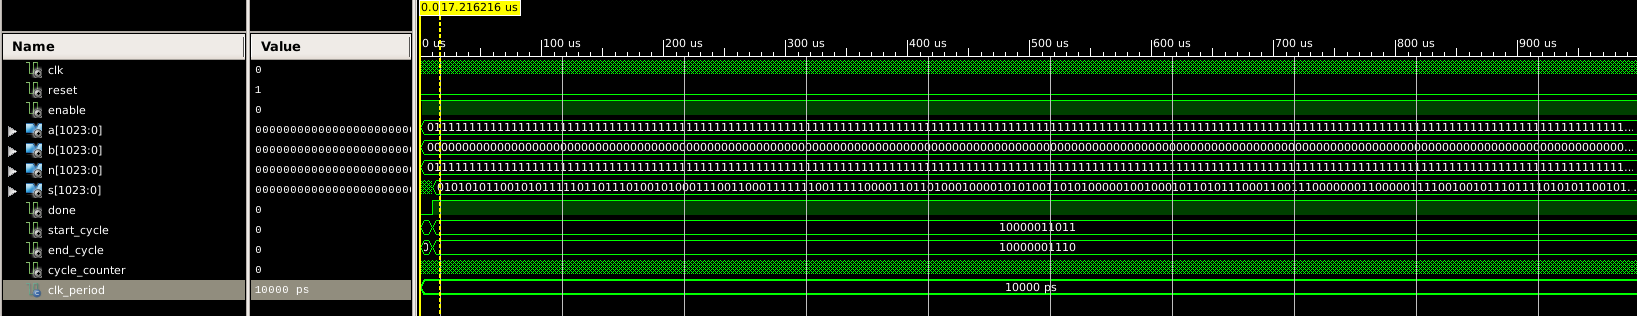
\includegraphics[width=0.65\textwidth]{figures/beispielbild.png}
  \caption{Beispielhafte Abbildung (eigene Darstellung).}
  \label{fig:beispiel}
\end{figure}

% -------- Absatz (A3) mit Verweis auf Grafik ----------
\begin{A3}
Abbildung~\ref{fig:beispiel} dient als schematisches Beispiel für die spätere Darstellung 
der Resultate. Sed cursus turpis vitae tortor. Donec posuere vulputate arcu. 
Phasellus accumsan cursus velit. Ut varius tincidunt libero. 
In hac habitasse platea dictumst.
\end{A3}

% -------- optionaler Absatz (A1) mit weiterem Zitat ----------
\begin{A1}
Zusammenfassend zeigt sich, dass die Kombination aus klarer Gliederung, 
präzisen Tabellen und erläuternden Abbildungen die Lesbarkeit steigert 
(vgl. erneut \cite{knuth1984}). Integer tincidunt. Cras dapibus. Vivamus elementum semper nisi.
\end{A1}
